%!TEX root = ../main.tex

\chapter{Application of the Model}\label{cha:applying-model}

\section{Memory1 Strategies}

\section{Determining the sensitivity of the Model}




\section{Applying Model to Axelrod-Python}


\begin{figure}[htbp!]
    \centering
    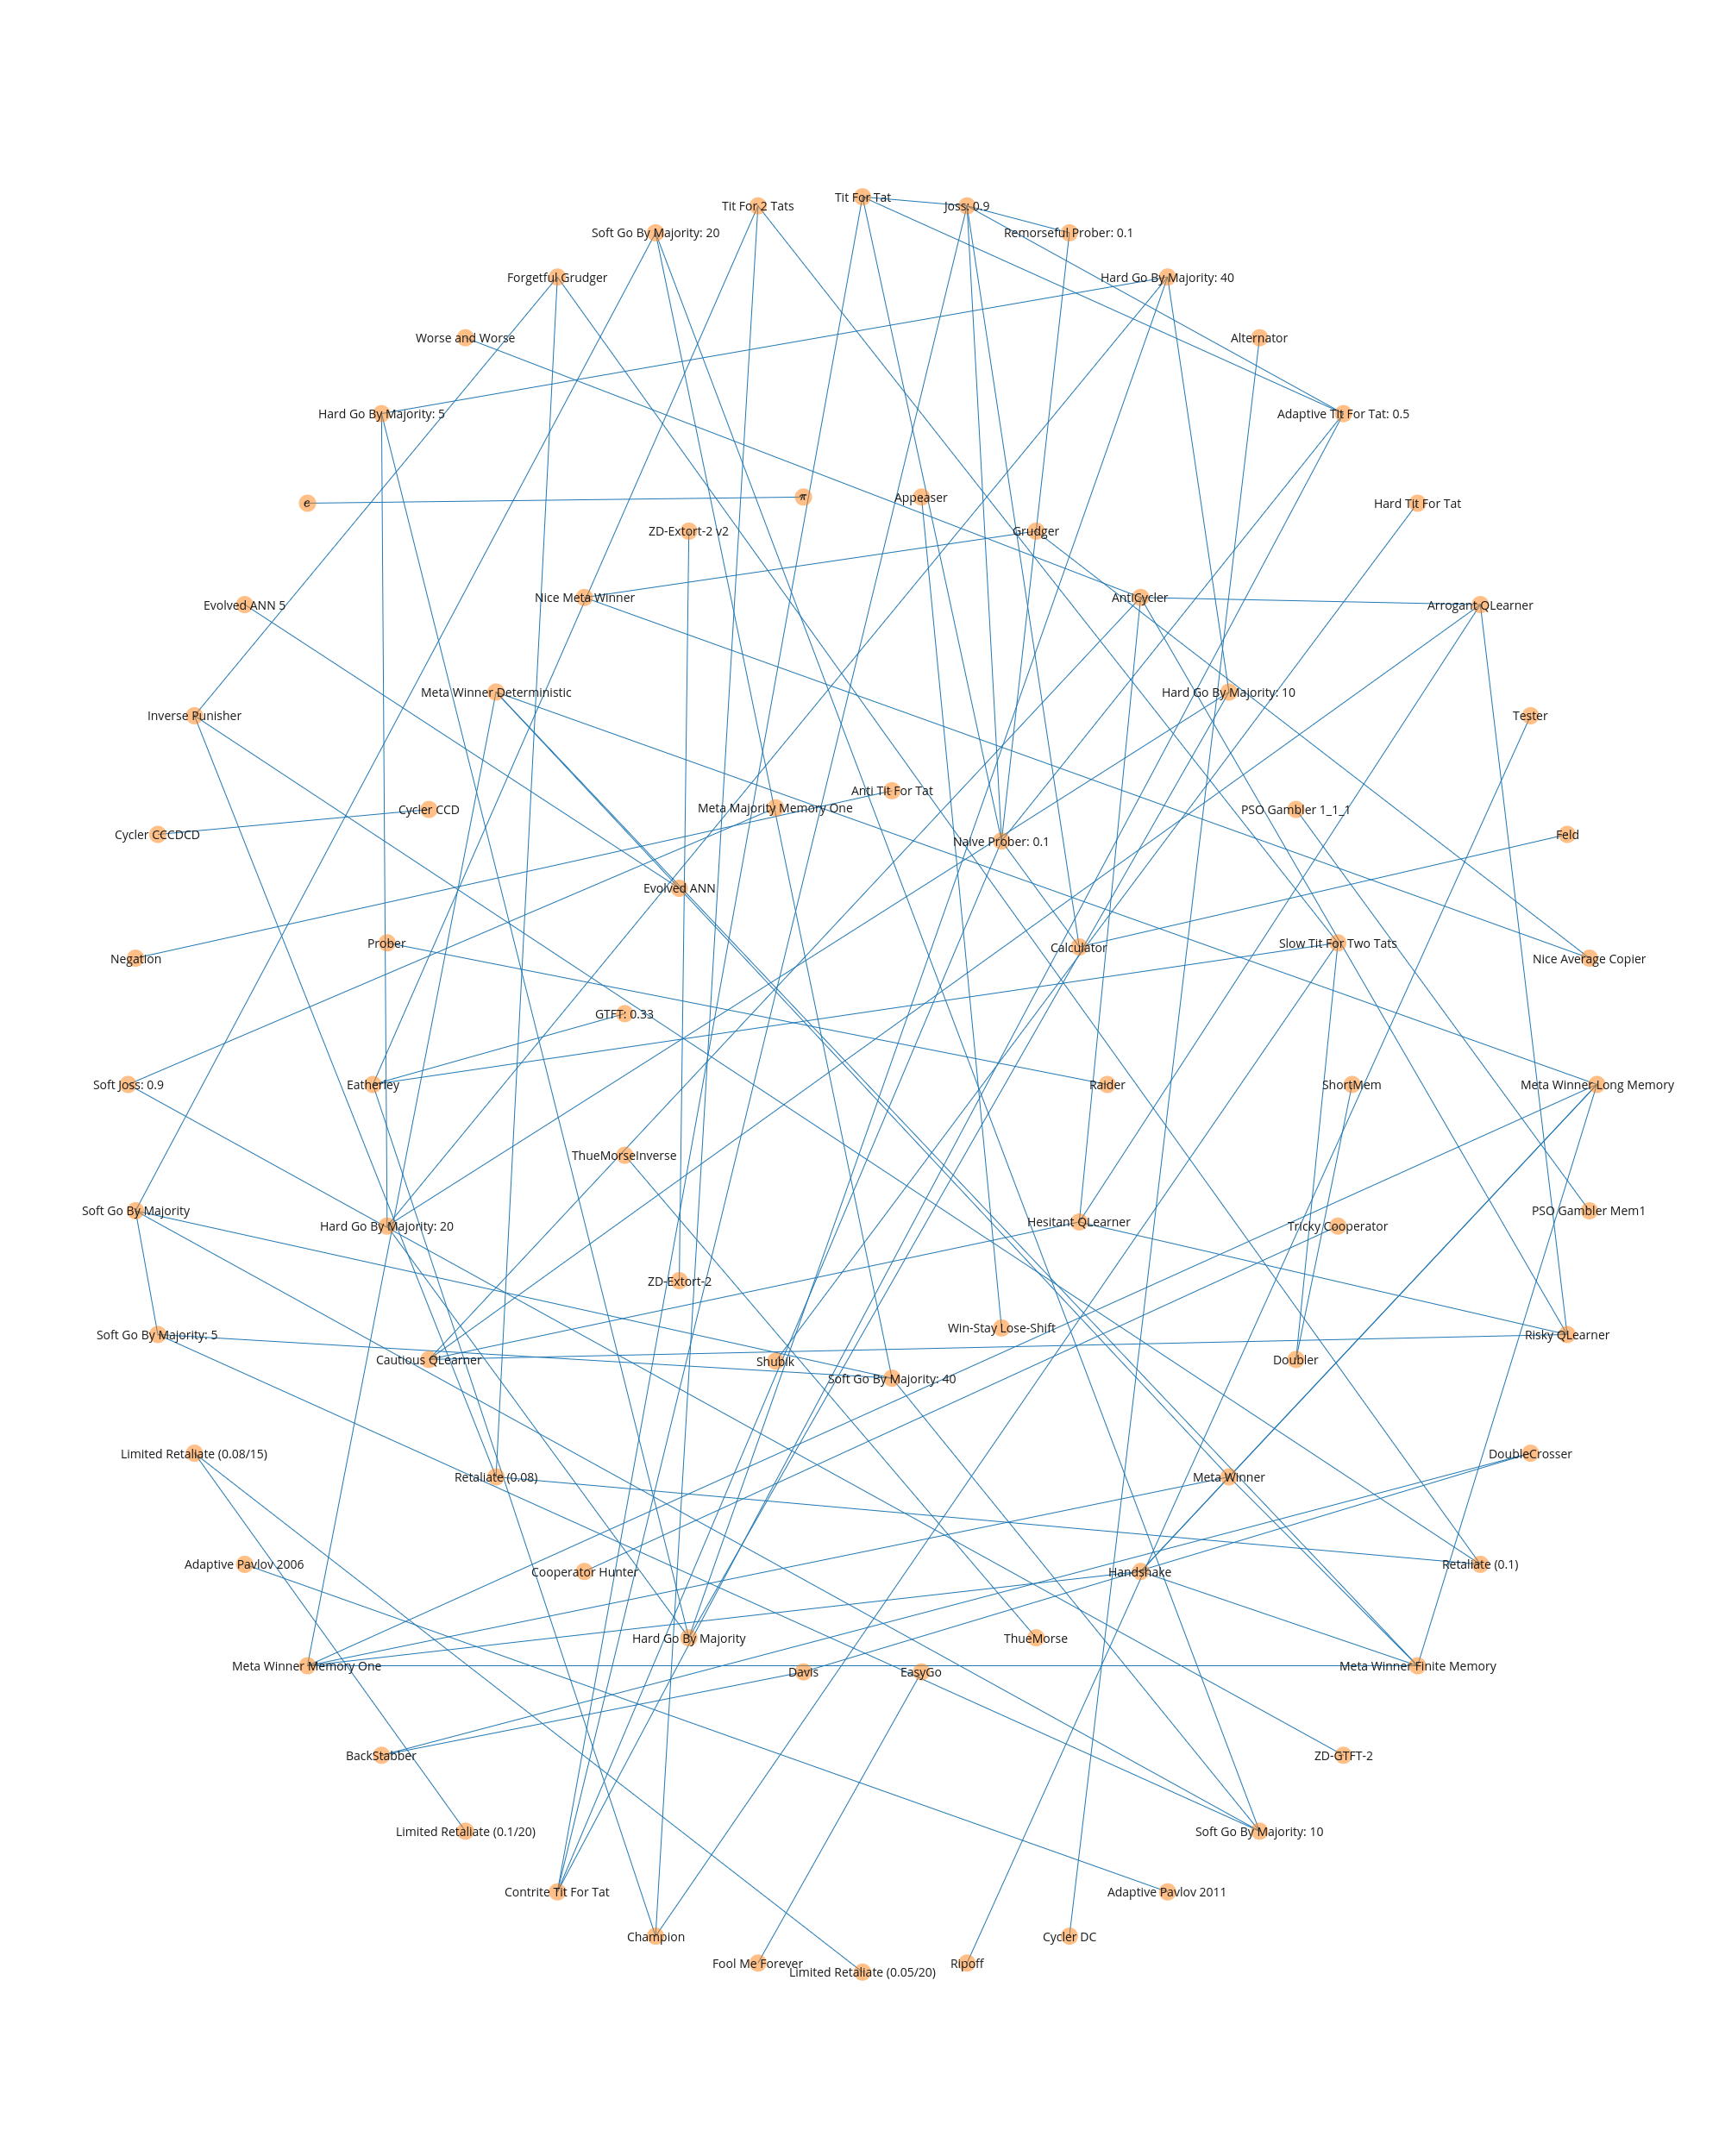
\includegraphics[width=\linewidth]{../img/neighbourhoods/overall.png}
    \caption{Caption here}
    \label{fig:figure1}
\end{figure}

\begin{figure}[htbp!]
\subfloat[]{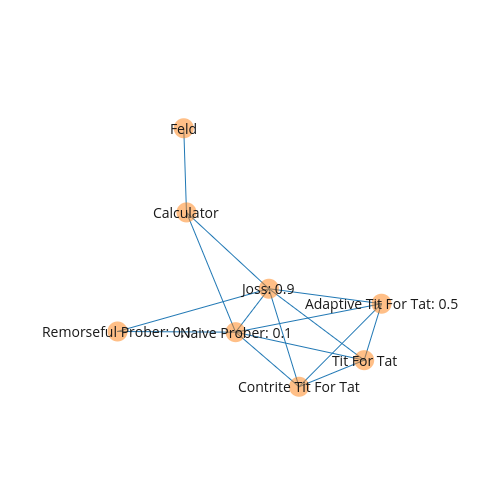
\includegraphics[width = 0.3\textwidth]{../img/neighbourhoods/1.png}}
\subfloat[]{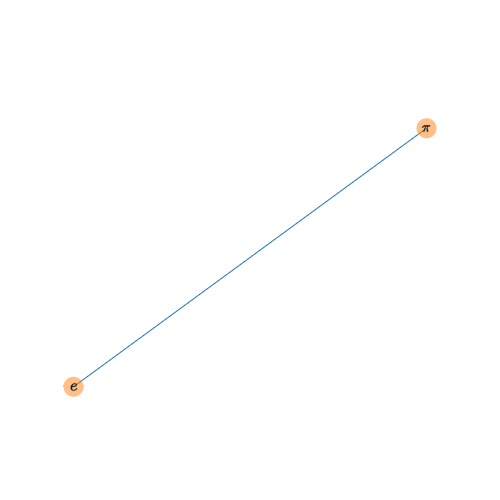
\includegraphics[width = 0.3\textwidth]{../img/neighbourhoods/10.png}}
\subfloat[]{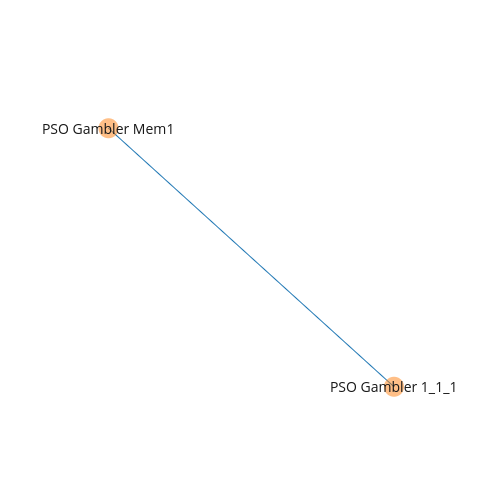
\includegraphics[width = 0.3\textwidth]{../img/neighbourhoods/102.png}} \\
\end{figure}
\begin{figure}[htbp!]
\ContinuedFloat
\subfloat[]{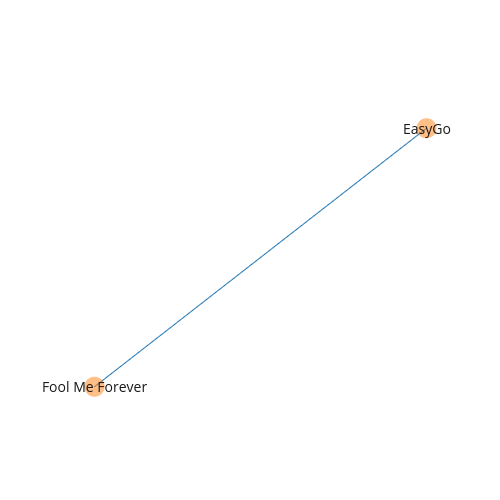
\includegraphics[width = 0.3\textwidth]{../img/neighbourhoods/107.png}}
\subfloat[]{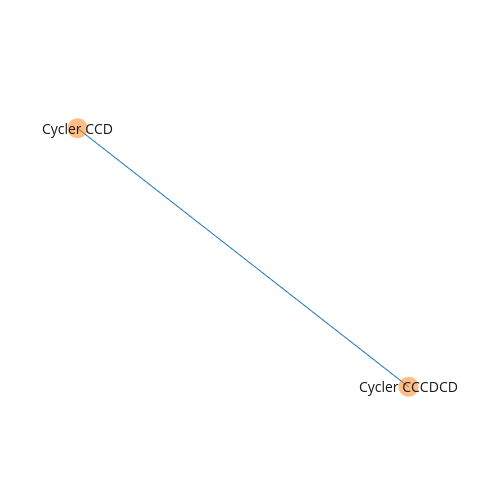
\includegraphics[width = 0.3\textwidth]{../img/neighbourhoods/12.png}}
\subfloat[]{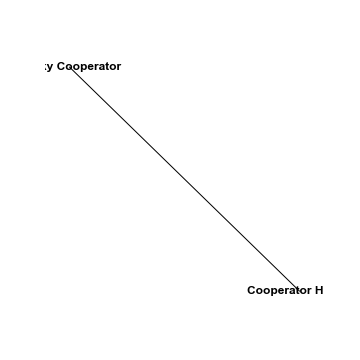
\includegraphics[width = 0.3\textwidth]{../img/neighbourhoods/16.png}} \\
\end{figure}
\begin{figure}[htbp!]
\ContinuedFloat
\subfloat[]{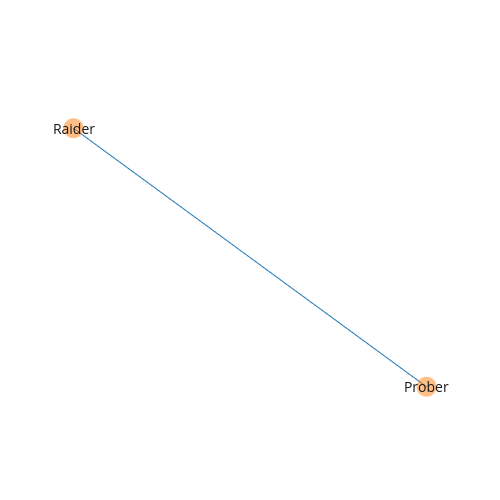
\includegraphics[width = 0.3\textwidth]{../img/neighbourhoods/17.png}}
\subfloat[]{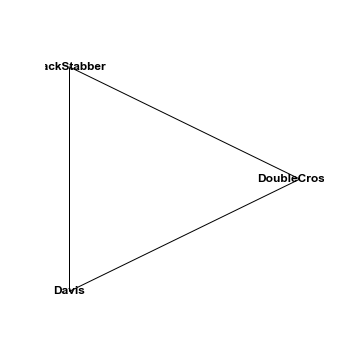
\includegraphics[width = 0.3\textwidth]{../img/neighbourhoods/18.png}}
\subfloat[]{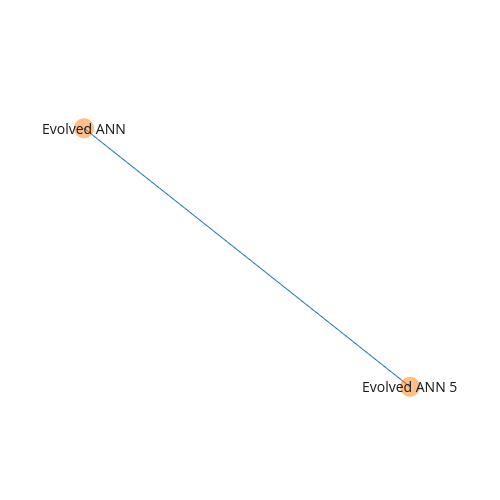
\includegraphics[width = 0.3\textwidth]{../img/neighbourhoods/2.png}} \\
\end{figure}
\begin{figure}[htbp!]
\ContinuedFloat
\subfloat[]{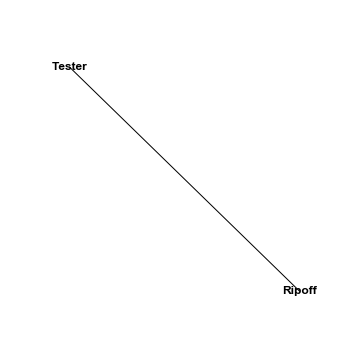
\includegraphics[width = 0.3\textwidth]{../img/neighbourhoods/22.png}}
\subfloat[]{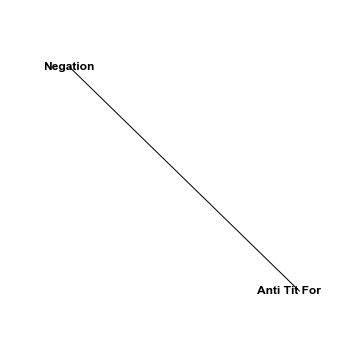
\includegraphics[width = 0.3\textwidth]{../img/neighbourhoods/24.png}}
\subfloat[]{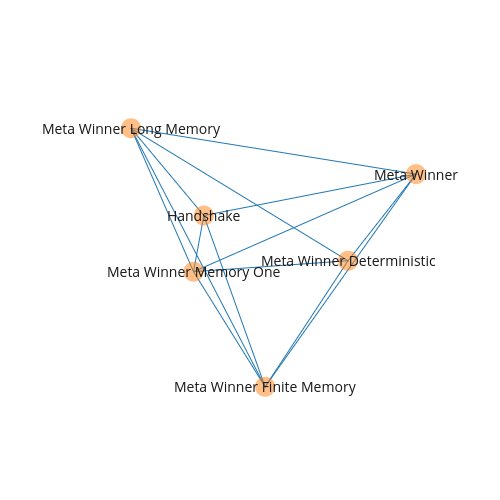
\includegraphics[width = 0.3\textwidth]{../img/neighbourhoods/29.png}} \\
\end{figure}
\begin{figure}[htbp!]
\ContinuedFloat
\subfloat[]{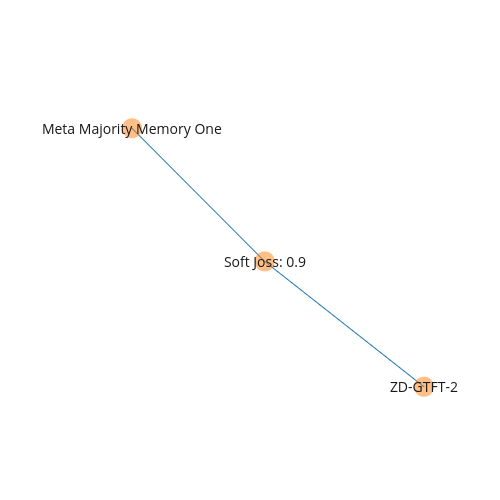
\includegraphics[width = 0.3\textwidth]{../img/neighbourhoods/30.png}}
\subfloat[]{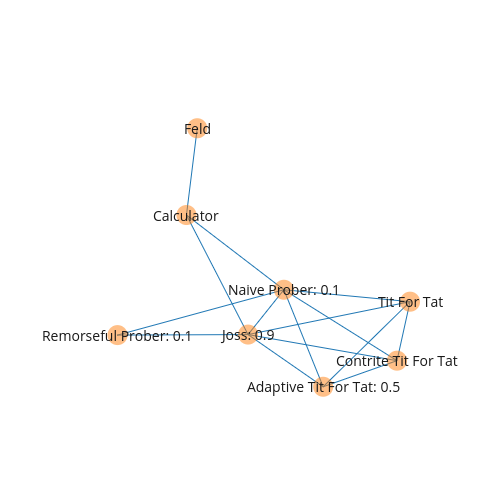
\includegraphics[width = 0.3\textwidth]{../img/neighbourhoods/31.png}}
\subfloat[]{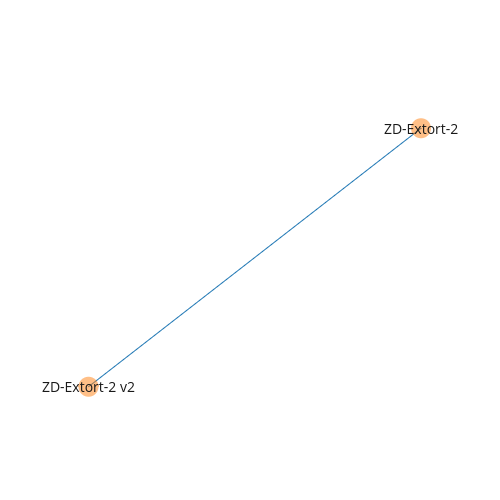
\includegraphics[width = 0.3\textwidth]{../img/neighbourhoods/36.png}} \\
\end{figure}
\begin{figure}[htbp!]
\ContinuedFloat
\subfloat[]{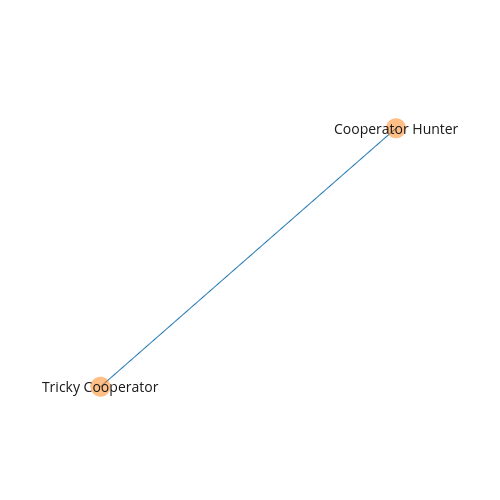
\includegraphics[width = 0.3\textwidth]{../img/neighbourhoods/38.png}}
\subfloat[]{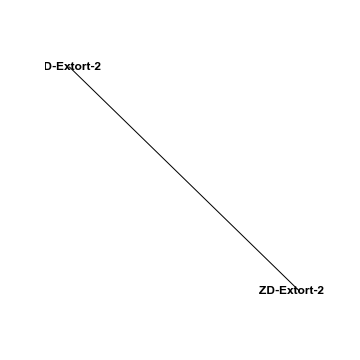
\includegraphics[width = 0.3\textwidth]{../img/neighbourhoods/4.png}}
\subfloat[]{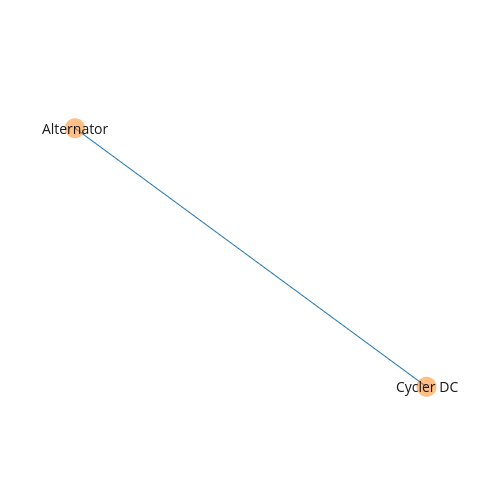
\includegraphics[width = 0.3\textwidth]{../img/neighbourhoods/47.png}} \\
\end{figure}
\begin{figure}[htbp!]
\ContinuedFloat
\subfloat[]{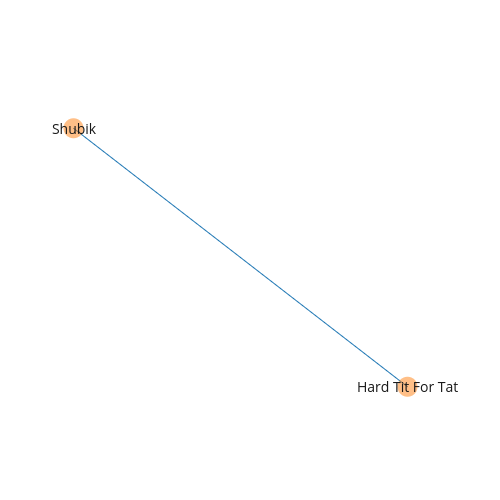
\includegraphics[width = 0.3\textwidth]{../img/neighbourhoods/49.png}}
\subfloat[]{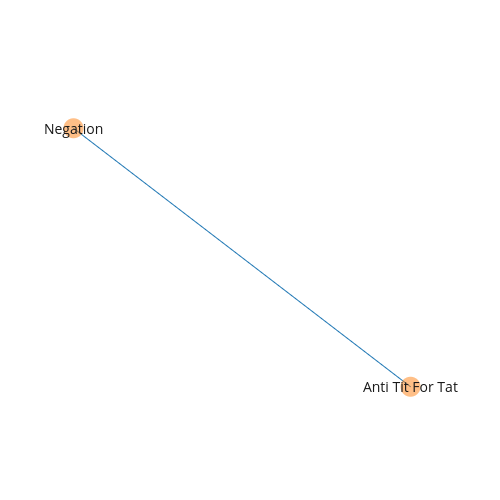
\includegraphics[width = 0.3\textwidth]{../img/neighbourhoods/55.png}}
\subfloat[]{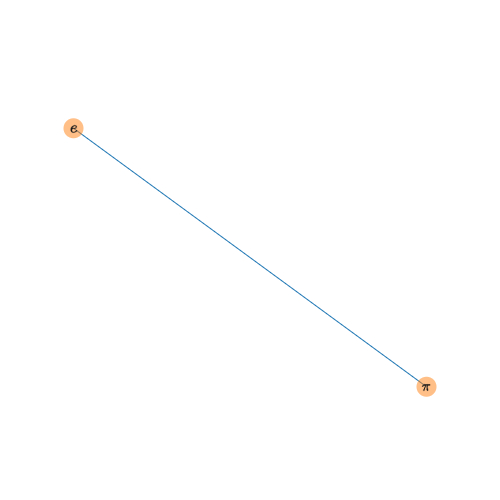
\includegraphics[width = 0.3\textwidth]{../img/neighbourhoods/58.png}} \\
\end{figure}
\begin{figure}[htbp!]
\ContinuedFloat
\subfloat[]{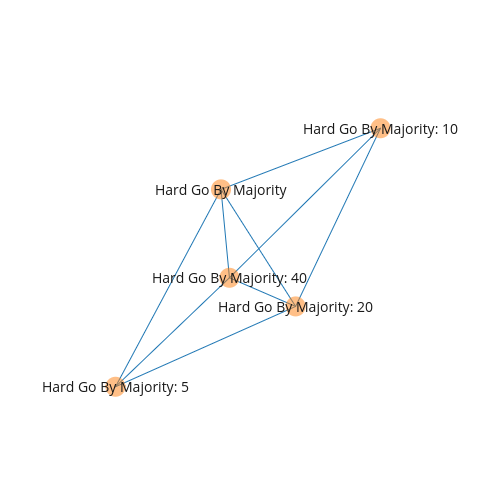
\includegraphics[width = 0.3\textwidth]{../img/neighbourhoods/60.png}}
\subfloat[]{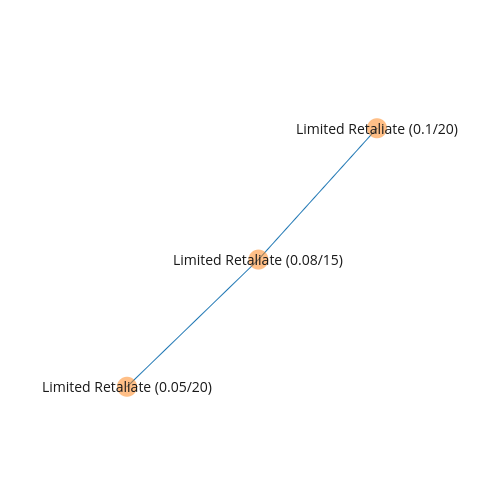
\includegraphics[width = 0.3\textwidth]{../img/neighbourhoods/7.png}}
\subfloat[]{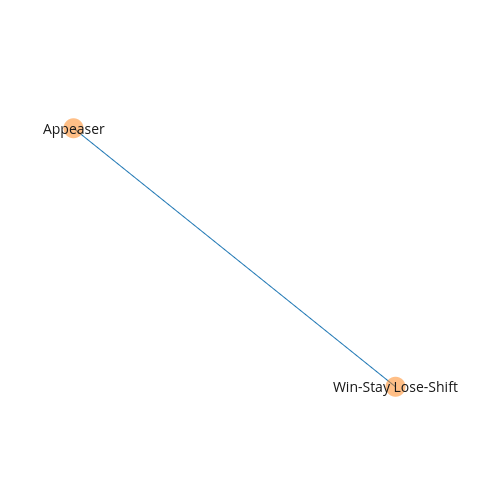
\includegraphics[width = 0.3\textwidth]{../img/neighbourhoods/74.png}} \\
\end{figure}
\begin{figure}[htbp!]
\ContinuedFloat
\subfloat[]{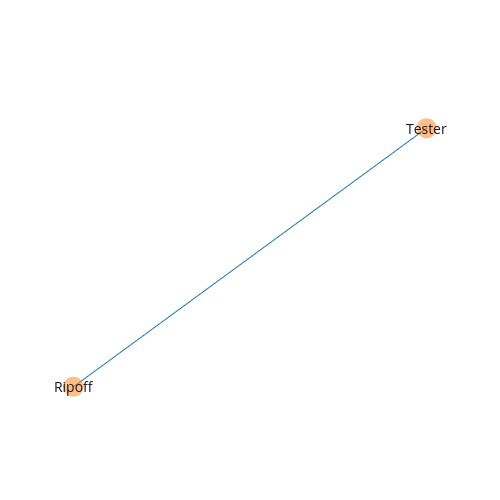
\includegraphics[width = 0.3\textwidth]{../img/neighbourhoods/78.png}}
\subfloat[]{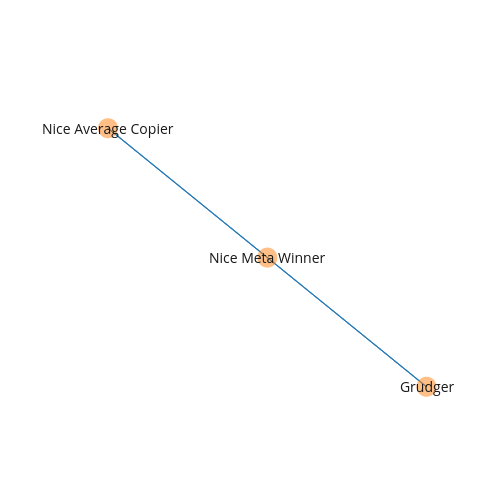
\includegraphics[width = 0.3\textwidth]{../img/neighbourhoods/84.png}}\\
\end{figure}
